\documentclass[12pt, twoside, letterpaper]{report}

\usepackage[top=2cm,bottom=4cm,left=3cm,right=3cm,asymmetric]{geometry}
\usepackage{fancyhdr}
\pagestyle{fancy}
\fancyfoot[C]{}    
\fancyfoot[LE,RO]{\thepage}        
\fancyhead[RO]{\slshape \rightmark}
\fancyhead[LE]{\slshape\leftmark}      
\fancyhead[RE,LO]{}

%pacchetti
\usepackage{color, xcolor}   
\usepackage{hyperref}
\usepackage[utf8x]{inputenc}
\usepackage[italian]{babel}
\usepackage{amsmath, amsthm, amssymb, amsfonts}
\usepackage{blindtext}
\usepackage{dirtytalk}
\usepackage{cite}
\usepackage[breakable]{tcolorbox}
\usepackage{pdfpages}
\usepackage{booktabs}
\usepackage{enumitem}
\usepackage{caption}
\usepackage{subcaption}
\usepackage{graphicx}

%Formattazione codice
\usepackage{listings}
\definecolor{codegreen}{rgb}{0,0.6,0}
\definecolor{codegray}{rgb}{0.5,0.5,0.5}
\definecolor{codepurple}{rgb}{0.58,0,0.82}
\definecolor{backcolour}{rgb}{0.95,0.95,0.92}

\lstdefinestyle{mystyle}{
    backgroundcolor=\color{backcolour},   
    commentstyle=\color{codegreen},
    keywordstyle=\color{magenta},
    numberstyle=\tiny\color{codegray},
    stringstyle=\color{codepurple},
    basicstyle=\ttfamily\footnotesize,
    breakatwhitespace=false,         
    breaklines=true,                 
    captionpos=b,                    
    keepspaces=true,                 
    numbers=left,                    
    numbersep=5pt,                  
    showspaces=false,                
    showstringspaces=false,
    showtabs=false,                  
    tabsize=2
}

\lstset{style=mystyle}

%Immagini
\graphicspath{ {./img/} }
\newcommand{\img}[4] {
	\begin{figure}
		\centering
		\includegraphics[scale=#2]{#3}\\
		\caption{#1}
		\label{fig:#4}
	\end{figure}
}
\newcommand{\imgh}[4] {
	\begin{figure}[h]
		\centering
		\includegraphics[scale=#2]{#3}\\
		\caption{#1}
		\label{fig:#4}
	\end{figure}
}



%%%%%%%%%%%%%%%%%%%%%%%%%%%%%%%%%%%%%%%%%%%%%%%%%%%%%%%%%%%%%%%%%%%%%%%%%%%%%%%%%%%%%%%%%%%%%%%%%%%%

\title{Uso di reti neurali per la classificazione di dati in problemi di medicina legale}
\author{Mario Petruccelli \cr Università degli studi di Milano}
\date{A.A. 2019/2020}

\begin{document}

	\begin{titlepage}
		
\includepdf{img/FRONTESPIZIO.pdf}
		\newpage
		\tableofcontents
		\thispagestyle{empty}
	\end{titlepage}

	\chapter*{Introduzione} \markboth{Introduzione}{}  \addcontentsline{toc}{chapter}{Introduzione}  \pagenumbering{arabic}
		Qua ci andrà l'introduzione

		\newpage		
	\chapter{Reti neurali}
		Le \textbf{reti neurali artificiali} sono un modello matematico molto importante del \textit{machine learning} che prende ispirazione dalle reti neurali biologiche presenti nel cervello animale. In questo Capitolo vedremo le componenti e il funzionamento delle reti neurali artificiali, ma prima facciamo un'overview su cosa sia il machine learning.

		\section{Paradigma del machine learning}
			Il machine learning è una branca dell'intelligenza artificiale ed è una di quelle in più rapida espansione; negli ultimi decenni è diventato di uso comune in moltissime applicazioni che richiedono l'estrazione di informazioni dai dati. Lo scopo del machine learning è quello di riassumere tante istanze di un problema, che difficilmente sarebbero riconoscibili con l'uso tradizionale della programmazione \textit{(per esempio riconoscere la razza di un cane partendo da una foto)}.   
			
			Prendendo come esempio noi umani, molte delle nostre abilità vengono acquisite o raffinate dalla nostra esperienza, e così \textit{apprendiamo}. Immaginiamo di trovarci davanti un essere vivente che non abbiamo mai visto prima. Nonostante questo essere sia nuovo ai nostri occhi, sapremo riconoscere con molta probabilità se questo si tratti di un insetto, di un mammifero o di una pianta. Lo stesso concetto possiamo provare ad applicarlo alle macchine, ma come possono apprendere? 
			
			\subsection{Tipi di apprendimento} Il machine learning è diviso in diversi sottocampi in cui abbiamo più paradigmi di apprendimento. La principale distinzione che si può fare è la differenza tra l'apprendimento \textbf{supervisionato}, \textbf{non supervisionato} e \textbf{per rinforzo}. Per quanto riguarda ciò che vedremo nei prossimi capitoli, possiamo concentrarci solo sulla differenza tra l'apprendimento supervisionato e non supervisionato.
			
				\paragraph{Apprendimento supervisionato} Consideriamo di dover classificare tre specie di fiori leggermente diversi tra loro appartenenti alla stessa famiglia \textit{(esperimento che riprenderemo più avanti)}. Per imparare a riconoscerli, potremmo ricevere un insieme di dati \textit{(per esempio la larghezza dei petali, lunghezza del gambo, ecc...)} che descrivono i fiori e cercare di predire la specie. Una figura d'insegnante (\textit{teacher}) ci da una \textbf{risposta d'apprendimento} per ogni tentativo che facciamo di indovinare l'\textbf{etichetta}, ovvero la classe di cui fanno parte. Dopo questa fase di \textbf{allenamento}, dovremmo essere stati in grado di aver trovato un pattern tra i dati per etichettare nuovi fiori, questa volta privi di etichetta e non appartenenti all'insieme dato in precedenza. 
										
					In maniera più astratta, possiamo vedere questo come un processo di \textit{utilizzo dell'esperienza passata per acquisire competenza}. L'apprendimento supervisionato descrive uno scenario in cui dobbiamo utilizzare l'esperienza acquisita tramite il processo di apprendimento con un insieme di dati (\textbf{insieme di training}) per \textbf{predire} un'informazione mancante. La bontà di questo processo la si può testare con un altro insieme (\textbf{insieme di test}) calcolando l'errore in base a quante etichette vengono predette in modo corretto. 
				
				\paragraph{Apprendimento non supervisionato}  Nell'apprendimento non supervisionato non c'è distinzione tra i dati di training e di test. Vengono processati i dati con lo scopo di produrre una versione compressa, o un \say{riassunto} di essi. Il clustering, overro il raggruppamento dei dati in sottoinsiemi con caratteristiche simili è una delle pratiche più usate in questo campo.\\\\
				Il modello di cui ci occuperemo noi, ovvero le reti neurali artificiali, utilizzano un'apprendimento di tipo supervisionato.
				
				
		\section{Che cos'è una rete neurale?}
			Il cervello animale è un meccanismo in grado di apprendere grazie all'esperienza, ed è per questo che si è cercato di emularlo \textit{(in modo molto semplificato)} come modello di machine learning. Il nucleo di tale organo sono i \textbf{neuroni}, ed essi sono connessi tra di loro tramite delle \textbf{sinapsi} in modo da poter comunicare. Ebbene, anche il modello artificiale riprende questa forma. L'archetipo matematico di neurone è stato ideato da McCulloch e Pitts nel 1943 \cite{mcculloch_pitts}. Lo descrivono come un modello contenente una soglia che ne determina lo stato di attivazione e una funzione non lineare detta \textbf{funzione di attivazione} che riceve uno o più input \textbf{pesati} e produce un unico output.
			
		\subsection{Componenti principali di una rete neurale} 
			\paragraph{Concetto di tempo} Prima di dare una definizione, introduciamo il concetto di tempo in una rete neurale. Ci si riferisce al tempo vigente come $(t)$, al passo successivo come $(t+1)$, al passo precedente come $(t-1)$, e così via. $t$ assume solo valori discreti.
			
			\paragraph{Rete neurale artificiale} Una rete neurale artificiale è formata da un insieme di \textbf{nodi} \textit{(neuroni)}, che elaborano le informazioni ricevute e trasmettono il risultato ai nodi successivi, e da \textbf{archi orientati pesati} \textit{(sinapsi)}. Più formalmente, una rete neurale è una tripla $(N,V, \omega)$ in cui:
			\begin{itemize}
				\item $N$ è l'insieme dei neuroni,
				\item $V = \{(i,j) | i,j \in N\}$ è l'insieme delle connessioni tra i neuroni $i$ e $j$, 
				\item $\omega: V \rightarrow \mathbb{R}$ è la funzione di peso, dove $\omega(i,j)$ è il peso della connessione tra i neuroni $i$ e $j$.  
			\end{itemize}
			Un neurone elabora i dati che gli arrivano tramite le sue connessioni. Questo accade attraverso tre funzioni: funzione di \textbf{propagazione}, funzione di \textbf{attivazione} e funzione di \textbf{uscita}.
			
			\img{Struttura di un neurone \cite{kriesel}}{0.4}{neurone.png}{neurone} 
			
			 \paragraph{Funzione di propagazione} Dato un neurone $j$, sia $I = i_1, \dots, i_k$ l'insieme dei neuroni ad esso connessi. L'output $o_{i_1}, \dots, o_{i_k}$ di questi neuroni viene preelaborato producendo un valore detto \textit{network input} net$_j$  che verrà poi elaborato dalla funzione di attivazione. Più precisamente il network input è calcolato come segue: $$net_j = f_{prop}(o_{i_1}, \dots, o_{i_k}, \omega(i_1,j), \dots, \omega(i_k,j))$$
			 	La funzione di propagazione più usata è la \textbf{somma pesata}, ovvero la somma delle moltiplicazioni dell'output di ogni neurone $i$ per il corrispettivo peso $\omega(i,j)$: $$net_j = \sum_{i \in I} o_i \omega(i,j)$$
			 	
			 \paragraph{Stato di attivazione e valore di soglia} Ad ogni istante un neurone può essere \textit{attivo} o meno. Lo \textbf{stato di attivazione} \textit{(o attivazione)} è una reazione ai valori ricevuti in input, e il neurone viene attivato quando il network input supera il \textbf{valore di soglia} di quel neurone. 
			 
			 Sia $j$ un neurone. Il \textbf{valore di soglia} $\Theta_j$ è assegnato unicamente a $j$ e rappresenta il punto di massima pendenza della funzione di attivazione, oltre il quale si considera $j$ attivo.
			 
			 
			 \paragraph{Funzione di attivazione} Sia $j$ un neurone. La funzione di attivazione è così definita: $$a_j(t) = f_{act}(net_j(t), \Theta_j)\footnote{In alcune reti neurali ricorsive è presente come parametro della funzione di attivazione anche il precedente stato di attivazione $a_j(t-1)$.}.$$ 
			 	In funzione del \textit{network input} net$_j$ e dell valore di soglia $\Theta_j$ ricava un nuovo stato di attivazione $a_j(t)$
			 	A differenza di molte delle variabili definite prima, la funzione di attivazione viene definita \textit{globalmente} per ogni strato di neuroni. Esistono diverse funzioni di attivazione, alcune tra le più usate, come possiamo vedere in figura~\ref{fig:funzioni di attivazione} sono: 
			 	\begin{itemize}
			 		\item la funzione logistica: $f(x) = \frac{1}{1+e^{-x}}$,
			 		\item la funzione tangente iperbolica: $f(x) = \tanh(x)$,
			 		\item la funzione ReLU: $f(x) = \max(0,x)$,
			 		\item la funzione identità: $f(x) = x$.
			 	\end{itemize}
			 \begin{figure}
				\begin{subfigure}[]{.5\textwidth}
					\centering
					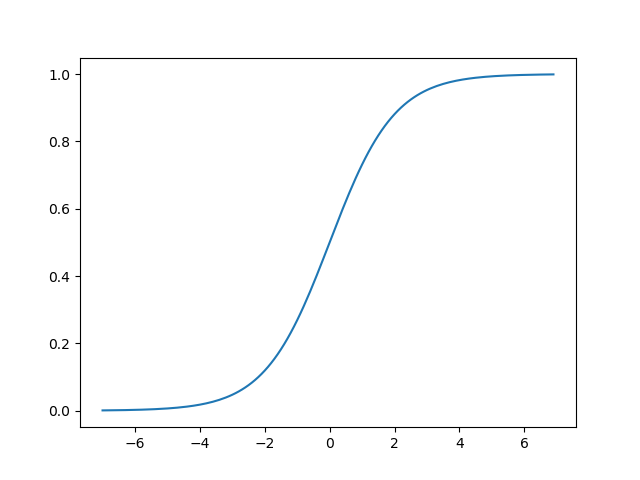
\includegraphics[width=.9\linewidth]{logistic.png}
					\caption{Funzione logistica}
					\label{fig:logistic}
				\end{subfigure}
				\hfill
				\begin{subfigure}[]{.5\textwidth}
					\centering
					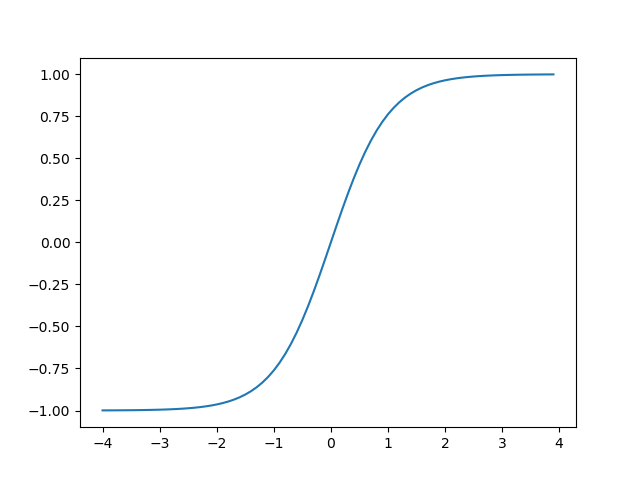
\includegraphics[width=.9\linewidth]{tanh.png}
					\caption{Funzione tangente iperbolica}
					\label{fig:tanh}
				\end{subfigure}
				
				\bigskip  
				
				\begin{subfigure}[]{.5\textwidth}
					\centering
					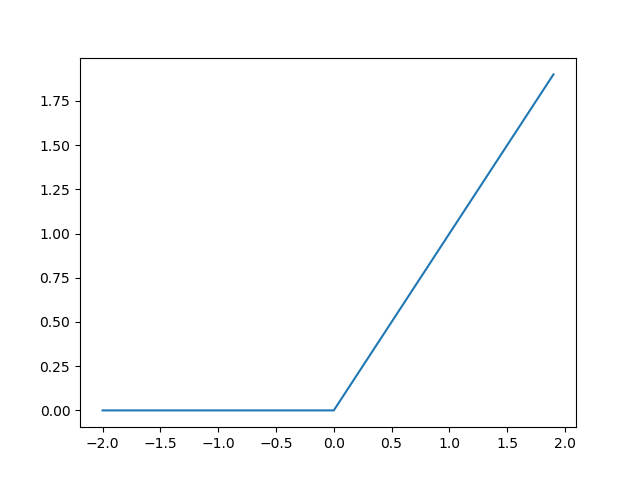
\includegraphics[width=.9\linewidth]{relu.png}
					\caption{Funzione ReLU}
					\label{fig:relu}
				\end{subfigure}
				\hfill
				\begin{subfigure}[]{.5\textwidth}
					\centering
					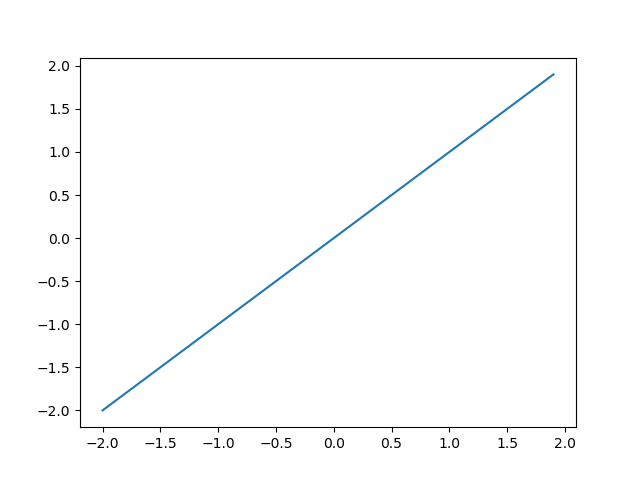
\includegraphics[width=.9\linewidth]{identity.png}
					\caption{Funzione di identità}
					\label{fig:identity}
				\end{subfigure}
				
				\caption{Funzioni di attivazione}
				\label{fig:funzioni di attivazione}
			\end{figure}	
			 	
			 \paragraph{Funzione di uscita} La funzione di uscita di un neurone $j$ calcola i valori che verranno trasmessi agli altri neuroni connessi a $j$. 
			 
			 	Sia $j$ un neurone. La funzione di uscita calcola il valore di output $o_j$ del neurone $j$ in funzione dell'attivazione $a_j$. $$o_j = f_{out}(a_j)$$  
			 	Anche in questo caso, solitamente la funzione è definita per ogni strato di neuroni. Spesso viene usata come funzione di uscita la \textit{funzione di identità}, mandando in output direttamente l'attivazione $a_j$. $$f_{out}(a_j) = a_j, \text{ quindi } o_j = a_j$$
			 	
			 \paragraph{Neurone bias} I valori di soglia $\Theta_{j_1}, \dots, \Theta_{j_n}$ dei neuroni $j_1, \dots, j_n$ possono essere realizzati come pesi di un neurone sempre attivo. Aggiungiamo quindi un neurone \textit{bias} il cui \textit{output} è fisso a 1, connesso ai neuroni $j_1, \dots, j_n$ il cui peso delle connessioni è pari a $-\Theta_{j_1}, \dots, -\Theta_{j_n}$. Questa semplificazione permette di facilitare i conti quando si derivano delle proprietà formali del modello.
			 
			 	\img{Due reti equivalenti, a destra con neurone bias e a sinistra senza. \cite{kriesel}}{0.5}{bias-neuron.png}{bias}
			 	
			 \paragraph{Vettore d'ingresso e vettore di uscita} Le reti neurali che andremo a vedere \textit{(cioè le reti neurali feed-forward)} fanno parte di quella categoria di reti che processano dei dati in input per poi produrre un output. Una rete con $n$ neuroni di ingresso, necessita di un \textbf{vettore d'ingresso} $x = (x_1, x_2, \dots, x_n)$ che gli verrà dato in input e fornisce un \textbf{vettore di uscita} $y = (y_1, y_2, \dots, y_m)$.  
			 	 			 
		\section{Reti neurali feed-forward}
			Esistono diverse topologie di rete, ma noi ci concentreremo sulle \textbf{reti neurali feed-forward} \textit{(o in italiano, reti neurali con flusso in avanti)}. In queste reti, i neuroni sono raggruppati in diversi \textbf{strati}: \textit{uno strato di ingresso, $k$ strati nascosti} e \textit{uno strato di uscita}. In una rete feed-forward ogni neurone ha connessioni dirette solo con lo strato successivo a quelli in cui è contenuto (in direzione dello strato di uscita), evitando così l'esistenza di cicli. Una rete feed-forward in cui ogni neurone è connesso a tutti i neuroni dello strato successivo viene detta rete \textbf{completamente connessa}.

			\paragraph{Percettrone} Un percettrone è una rete feed-forward completamente connessa costituita da uno strato d'ingresso in cui i neuroni di input propagano l'informazione ricevuta \textit{(cioè le funzioni di propagazione, attivazione e uscita del primo strato di neuroni sono la funzione identità)}, seguito da almeno uno strato di pesi addestrabili.
			
			\paragraph{Percettrone a singolo strato} Un percettrone a singolo strato è il percettrone più semplice che si possa fare. Esso è costituito da uno strato di neuroni d'ingresso e uno di uscita. 
				\img{Percettrone a singolo strato con 5 neuroni di ingresso e 3 neuroni di uscita. \cite{kriesel}}{0.5}{slp.png}{slp} 
				
			\paragraph{Separabilità lineare} Siano $X$ e $Y$ due insiemi $\in \mathbb{R}^b$. Essi sono linearmente separabili se e solo se esiste un iperpiano $P$ di $\mathbb{R}^b$ tale che gli elementi di $X$ e $Y$ sono divisi da $P$. 
			
			\begin{figure}
				\begin{subfigure}[]{.5\textwidth}
					\centering
					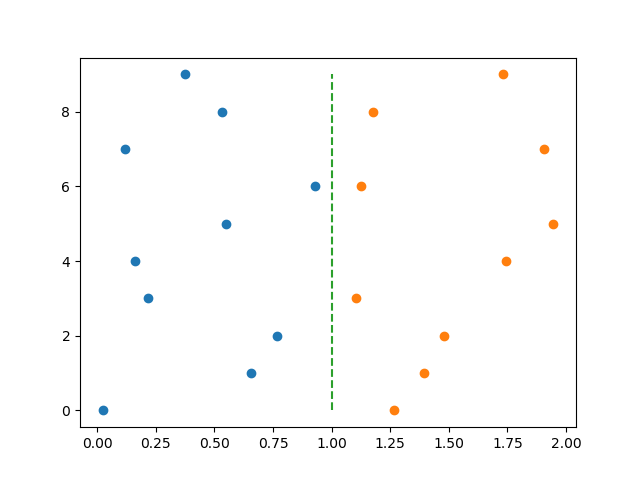
\includegraphics[width=.9\linewidth]{linearly_separable.png}
					\caption{Dati separabili linearmente}
					\label{fig:linearly_separable}
				\end{subfigure}
				\hfill
				\begin{subfigure}[]{.5\textwidth}
					\centering
					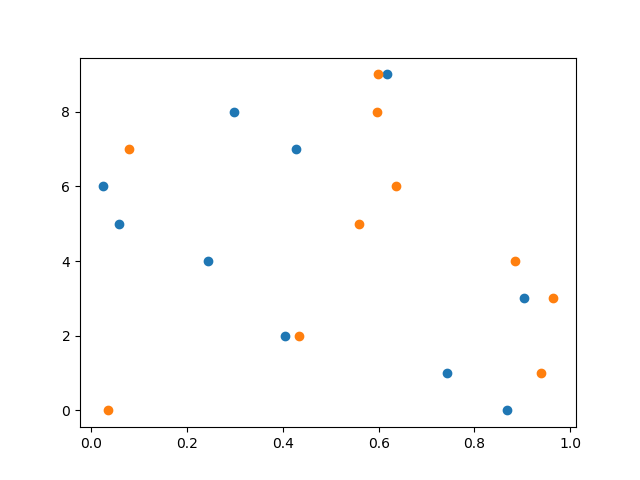
\includegraphics[width=.9\linewidth]{not_linearly_separable.png}
					\caption{Dati \textbf{non} separabili linearmente}
					\label{fig:not_linearly_separable}
				\end{subfigure}
				
				\caption{Separabilità lineare}
			\end{figure}	

				
				 
			\paragraph{Percettrone multistrato} Un percettrone multistrato è un percettrone con più di uno strato di pesi addestrabili. M. Minsky e S. Papert nel 1969 \cite{minsky_papert} dimostrarono che i percettroni a singolo strato sono in grado di approssimare solo funzioni che separano i dati \textbf{linearmente}; i percettroni multistrato ci permettono di aggirare questa limitazione. 
				\img{Percettrone multistrato. \cite{kriesel}}{0.5}{nn-feed-forward.png}{feedforward}
		
		\section{Apprendimento di una rete neurale}
			Abbiamo visto la struttura delle reti neurali ma ancora non sappiamo niente su come esse apprendano. Sappiamo che in una rete feed-forward ogni neurone è collegato tramite degli archi pesati a tutti i neuroni dello strato successivo, ma non sappiamo come i pesi vengano inizializzati e in base a cosa vengano modificati. In realtà il processo di apprendimento può essere descritto in pochi passi: 
			\begin{enumerate}
				\item inizializzare i pesi della rete neurale in modo casuale,
				\item dare in input alla nostra rete un vettore d'ingresso $p$ di cui sappiamo l'etichetta,
				\item propagare in avanti l'input fino ai neuroni di uscita attraverso le tre funzioni viste prima, 
				\item siano $y$ il vettore di uscita ottenuto e $t$ il vettore di uscita desiderato: sottraendo i due vettori otteniamo un \textbf{vettore di errore} $E_p = t - y$,
				\item correggere i pesi con lo scopo di ridurre al minimo $E_p$,
				\item reiterare 2-5 finchè non si raggiunge un errore soddisfacente.
			\end{enumerate}
			Questo è un processo iterativo su due dimensioni. Si itera più volte (finchè non consideriamo l'errore soddisfacente) su tutti i dati. Nonostante la differenza del vettore di errore converga verso un valore basso, questo non ci garantisce che la rete abbia appreso il pattern che c'è dietro ai dati, anzi, potrebbe aver imparato a riprodurre l'output dei dati che gli abbiamo dato in ingresso. Questo fenomeno è chiamato \textbf{overfitting} e per accorgerci di questo problema è buona prassi dividere in due insiemi i dati che usiamo per allenare la rete neurale in: 
			%fondere curva di apprendimento e altro (in monitorare) e aggiungere la parte qua sopra dopo che ci si pone il problema se ha generalizzato
			\begin{itemize}
				\item un insieme di \textbf{training} utilizzato per allenare la rete,
				\item un insieme di \textbf{test} utilizzato per valutare la bontà della rete.
			\end{itemize}
			Una \textit{best practice} è quella di dividere in modo casuale i dati talché siano influenzati il meno possibile da fattori esterni \textit{(per esempio prendere i primi dati in un dataset in cui essi sono ordinati in ordine crescente potrebbe influire negativamente sull'apprendimento)} e solitamente si tiene una proporzione in cui l'insieme di training ha un numero di dati maggiore rispetto all'insieme di test (almeno 3/4 dei dati totali). 

			\paragraph{Apprendimento online e offline} Oltre alla principale distinzione vista in precedenza tra i tipi di apprendimento (supervisionato e non supervisionato), c'è un'altra distinzione importante sulla frequenza della modifica dei pesi. L'apprendimento può essere: 
				\begin{itemize}
					\item \textbf{Online:} i dati di training vengono inseriti uno a uno, la rete calcola l'errore del singolo dato e modifica i pesi di conseguenza.
					\item \textbf{Offline:} Tutti i dati di training vengono inseriti nella rete insieme, la rete accumula gli errori e modifica i pesi di conseguenza. Ogni lotto di dati viene detto \textbf{batch}, e tutta la procedura di apprendimento dell'intero insieme viene detta \textbf{epoca}.
				\end{itemize}
				Esiste anche una via di mezzo in cui i dati vengono divisi in \textbf{mini-batch}, ovvero sottoinsiemi dell'insieme di training. Dati $h$ dati di training e una dimensione di batch $b$, in ogni epoca i pesi vengono ricalcolati $\lceil h/b \rceil$ volte.
			
			\subsection{Monitorare l'apprendimento di una rete neurale}
				Un modo spesso usato per monitorare l'apprendimento di una rete neurale è quello di tracciare \textbf{curva di apprendimento}. Essa traccia il progresso dell'errore e ci aiuta a capire se la nostra rete stia facendo progressi o meno. Per questo scopo normalizziamo l'errore in modo tale che sia sempre un valore positivo. Il modo più comune è quello di calcolare il valore efficace tra il vettore di uscita desiderato $t$ e il vettore di uscita $y$. 

				Siano $\Omega$ i neuroni di uscita, $O$ l'insieme dei neuroni di uscita e $P$ l'insieme di training. Il valore efficace del singolo elemento di training $p$ si calcola nel seguente modo: $$Err_p = \sqrt{\frac{\sum_{\Omega \in O} (t_{\Omega} - y_{\Omega})^2}{|O|}}.$$
				Per quanto riguarda l'apprendimento offline, l'\textbf{errore totale} di un'epoca si calcola nel seguente modo: $$Err = \sum_{p \in P} \frac{Err_p}{|P|}.$$ 
				La curva di apprendimento va tracciata per i due insiemi di training e test, in questo modo possiamo accorgerci se siamo in un caso di overfitting guardando solo l'andamento delle due curve: se la curva di training decresce velocemente mentre quella di test comincia a risalire siamo chiaramente in un caso in cui stiamo perdendo la generalizzazione dei dati che avevamo acquisito, l'ideale sarebbe fermarsi appena prima che la curva di test cominci a risalire (\textbf{early stopping}). Solitamente la curva di training avrà comunque un errore minore rispetto quella di test.

				\begin{figure}
				\begin{subfigure}[]{.5\textwidth}
					\centering
					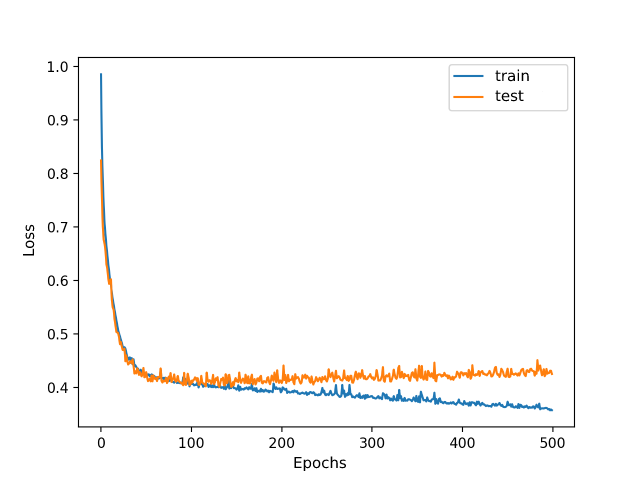
\includegraphics[width=\linewidth]{learning_curve.png}
					\caption{Curva di apprendimento regolare}
					\label{fig:learning_curve}
				\end{subfigure}
				\hfill
				\begin{subfigure}[]{.5\textwidth}
					\centering
					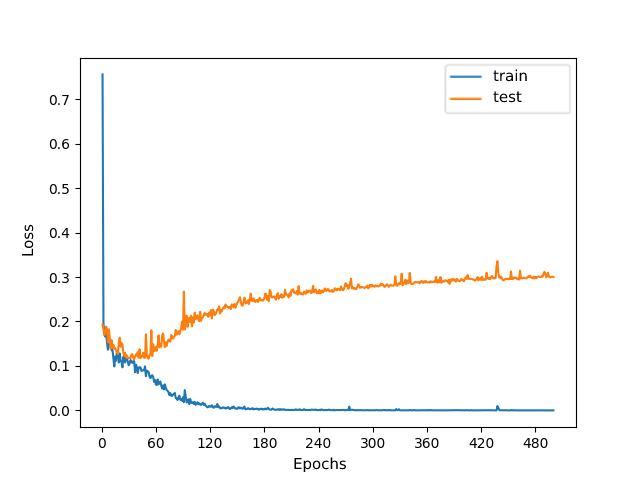
\includegraphics[width=\linewidth]{overfitting.png}
					\caption{Curva di apprendimento con overfitting}
					\label{fig:overfitting}
				\end{subfigure}
				
				\caption{Curve di apprendimento degli insiemi di training e test}
				\label{fig:curve_di_apprendimento}
				\end{figure}
				
			\subsection{Discesa del gradiente}
				Quando smettiamo di apprendere? Non è una domanda dalla risposta facile, e per capire questo fondamentale passaggio bisogna avere un'idea chiara di cosa sia la discesa del gradiente (figura \ref{fig:gradient_descent}). È una procedura che viene utilizzata per massimizzare o minimizzare una funzione. Con \say{discesa} e \say{salita} si intendono le direzioni che determinano il massimo aumento e la massima diminuzione di tale funzione. Il gradiente è un vettore $g$ definito in ogni punto derivabile di una funzione ed esso punta verso la salita più ripida. Di conseguenza $-g$ punterà verso la discesa più ripida.
				
				\img{Discesa del gradiente di una funzione a due dimensioni. \cite{kriesel}}{0.5}{gradient_descent_2d.png}{gradient_descent}
				
				\paragraph{Gradiente} Sia $f$ una funzione di $n$ argomenti, e $(x_1, \dots, x_n)$ un punto in cui essa è derivabile. Il gradiente di $f$ in $(x_1, \dots, x_n)$, indicato come $\nabla f(x_1, \dots, x_n)$, è il vettore di $n$ componenti ognuna delle quali è uguale a una delle derivate parziali di $f$: 
					$$\nabla f_i(x_1, \dots, x_n) = \frac{\partial f(x_1, \dots, x_n)}{\partial x_i}.$$
					In generale, $\nabla f(x_1, \dots, x_n)$ rappresenta la direzione verso cui spostarsi a partire da $(x_1, \dots, x_n)$ per massimizzare $f$, o, equivalentemente, per identificare la salita più ripida nel suo grafico. La norma $||\nabla f(x_1, \dots, x_n)||$ indica la pendenza di questa salita.
					
				%Anche dopo, quando parli della discesa del gradiente, è meglio continuare a fare riferimento a (x_1, \dots, x_n); inoltre attento a non confondere "dimensioni" con "argomenti". Attento anche che non è assolutamente detto che spostarsi nella direzione del'anti-gradiente garantisca ogni volta di avere valori minori di f, appunto per i problemi di cui tu stesso parli. In ogni caso non dire che il passo da fare a ogni iterazione è uguale alla norma del gradiente, quello è il miglior modo per divergere :-) Normalmente si usano dei passi di piccola ampiezza.

				\paragraph{Discesa del gradiente} Sia $f$ una funzione a $n$ argomenti e $x_1, \dots, x_n$ il dato punto di partenza. \textbf{Discesa del gradiente} significa andare da $f(x_1, \dots, x_n)$ in direzione di $-g$. L'idea è quella di andare verso valori sempre minori di $f$, anche se purtroppo questo non succede sempre.
								
				\img{Problemi della tecnica della discesa del gradiente \cite{kriesel}}{0.4}{gradient_descent.png}{gradient_descent_problemi}
				
				I motivi per cui questa tecnica potrebbe fallire sono diversi, alcuni esempi sono: 
				\begin{itemize}
				 	\item incagliarsi su un minimo locale non soddisfacente (Figura \ref{fig:gradient_descent}a),
				 	\item rallentare la ricerca del minimo a causa di un \textit{plateau} (Figura \ref{fig:gradient_descent}b),
				 	\item trovare un \say{canyon stretto} e continuare ad oscillare a causa dell'elevato contrasto tra i gradienti (Figura \ref{fig:gradient_descent}c),
				 	\item saltare un buon minimo a causa di una pendenza elevata (Figura \ref{fig:gradient_descent}d).
				 \end{itemize} 
				 
				 
			\subsection{Backpropagation}
				%Io propongo di spostare la parte "funzione di errore" dentro a 1.4.3 e di spiegare che un modo per indurre da dati etichettati una rete neurale è quello di inizializzare in qualche modo i pesi delle sue connessioni, poi presentarle alcuni esempi e calcolare l'errore corrispondente: l'algoritmo di backpropagation permette di legare il valore di errore contenuto al gradiente della funzione Err, così da poter applicare l'algoritmo della discesa del gradiente. In questo modo è possibile modificare per passi successivi i pesi delle connessioni, procedendo via via a diminuire l'errore. Quando questo è sotto una soglia accettabile, ciò significa che la rete neurale ottenuta classifica abbastanza bene gli esempi che le abbiamo fornito.

				%Ci sarebbe da spiegare poi, senza entrare in dettagli matematici ma facendo riferimento alla letteratura, che l'algoritmo di discesa del gradiente viene applicato in fasi successive: prima in modo da aggiornare i pesi delle connessioni che arrivano allo strato di output, e poi procedendo a ritroso nei vari strati (è per questo che si chiama backpropagation: l'errore viene propagato al contrario rispetto al verso di esecuzione della rete neurale).

					
				\paragraph{Funzione di errore} Ciò che noi vogliamo minimizzare è l'errore totale, ma per come l'abbiamo definito prima non è una funzione, quindi non sarebbe applicabile la discesa del gradiente. L'errore totale cresce o decresce in base a come cambiamo i pesi, quindi possiamo ridefinirlo come una \textbf{funzione di errore} che calcola l'errore normalizzato in funzione dei pesi $$Err : W \rightarrow \mathbb{R}$$ 
				 %$$\Delta \omega(i,\Omega) = \nu \cdot o_i \cdot \delta_{\Omega}.$$

				
				
	\chapter{Tecniche utilizzate}
		In questo Capitolo verrà fatta una panoramica sulle tecniche di \textbf{preprocessing}, \textbf{model selection} e \textbf{over-sampling} utilizzate negli esperimenti svolti. Questo aiuterà a capire con più facilità ciò di cui si parlerà nel Capitolo \ref{chap:esperimenti}.
		\section{Preprocessing}
			Nel machine learning, il preprocessing dei dati è uno step facoltativo (anche se solitamente aumenta notevolmente le performance) in cui si trasformano e/o codificano i dati con l'idea di renderli più facili da elaborare da parte dell'algoritmo di apprendimento utilizzato. In un dataset, i dati sono rappresentati da delle \textbf{feature}; esse possono essere di vari tipologie, tra cui quelle: 
			
			\begin{itemize}
				\item \textbf{categoriche:} rappresentano quelle caratteristiche i cui valori descrivono una qualità, e fanno solitamente parte di un insieme ben definito in cui il numero di valori è solitamente fissato \textit{(ad esempio i valori booleani: true, false; i colori: rosso, verde, blu, ecc...)},
				\item \textbf{numeriche:} rappresentano quelle caratteristiche i cui valori sono rappresentati da numeri con cui è possibile fare calcoli \textit{(ad esempio i numeri reali, i numeri naturali, ecc...)}.
			\end{itemize}
			Esistono diverse tecniche di preprocessing, ma nel seguito ci concentreremo solo su quelle che useremo durante gli esperimenti.
			
			\subsection{Riduzione della dimensionalità} In un dataset la dimensionalità è il numero di feature presenti. Con riduzione della dimensionalità si intende quell'insieme di tecniche che mirano a ridurre questo valore producendo una versione più compressa dei dati o eliminando delle feature. Queste tecniche vengono spesso utilizzate per visualizzare un insieme di dati in dimensionalità comode per le persone (solitamente 2 o 3 dimensioni) o per aiutare un modello predittivo a essere più efficiente e ad ignorare informazioni ridondanti o pressoché inutili che non aiutano, o peggio rendono più difficile, il processo di apprendimento. 
			
				\subsubsection{Feature selection e feature engineering} La feature selection è quel sottoinsieme di tecniche di riduzione della dimensionalità che include la completa rimozione di alcune feature dall'intero dataset. I modi in cui scegliere quali feature filtrare sono diversi: variano dalle analisi statistiche \textit{(ad esempio eliminare le feature con varianza minore)} ad analisi sull'accuratezza del modello predittivo. Una buona feature selection, oltre a rendere più veloce la fase di apprendimento, tende ad aumentare l'accuratezza del modello. %aggiungi una frase sulla feature engineering, spiegando che ti sei concentrato solo su quest'ultima, e in particolare sulle tecniche descritte subito dopo.
				
				\subsubsection{Analisi delle componenti principali} L'analisi delle componenti principali o \textbf{PCA} \textit{(da Principal Component Analysis)} è una tecnica di riduzione della dimensionalità dei dati che punta a ridurre le feature in una loro versione più compressa, evidenziandone le cosiddette componenti principali (caratterizzate dal fatto di massimizzare la varianza). Il tutto avviene tramite una \textbf{trasformazione lineare} dei dati, il cui risultato viene proiettato su una dimensione uguale o inferiore.
				\img{Proiezione dei dati da due a una dimensione con PCA \cite{bitsofdna}}{0.3}{pca.jpg}{pca}
				Sia $X$ una matrice con $n$ righe e $m$ colonne in cui ogni riga $x_i$ corrisponde a una misurazione diversa di un esperimento.  Per applicare la sopra menzionata trasformazione lineare, si calcola inizialmente la media delle righe 
				$$\overline{x}= \frac{1}{m} \sum_{j=1}^m x_j$$ 
				e si crea una matrice $\overline{X}$ con $n$ righe, ognuna delle quali è uguale a $\overline{x}$. Si sottraggono le matrici $X$ e $\overline{X}$ ottenendo così una matrice $B$ in cui la media di ogni riga è centrata in zero
				$$B = X - \overline{X}.$$
					 Si calcola successivamente la matrice di covarianza $C$ delle righe di $B$
					 $$C = B^\top B$$
					 e da $C$ si ricavano gli autovalori e gli autovettori $e_1, \dots, e_m$ che vengono allineati in ordine non crescente rispetto ai corrispondenti autovettori al fine di formare una matrice $E$; si ottengono così le direzioni dello spazio in cui è via via più alta la varianza dei dati osservati, e si considerano tali direzioni per costruire un nuovo sistema di assi cartesiani. Il prodotto $B \cdot E$ permette di ottenere la descrizione dei punti del dataset rispetto a questo nuovo sistema di assi e tenuto conto di come sono state ordinate le colonne di E, se vogliamo ridurre le dimensioni a un numero fissato $k$, allora dovremo eliminare da $E$ le ultime $m-k$ colonne, ottenendo così una matrice con le $k$ componenti principali.  	 
				
				\subsubsection{t-Distributed Stochastic Neighbor Embedding} t-Distributed Stochastic Neighbor Embedding (\textbf{t-SNE}) è una tecnica non lineare di riduzione della dimensionalità, presentata per la prima volta nel 2008 da  L.J.P. van der Maaten e G.E. Hinton \cite{maaten_hinton}. Tale algoritmo, introdotto per permettere la visualizzazione bi- o tridimensionale di dati complessi, può anche essere usato come metodo per la riduzione della dimensionalità.
				
					\img{Visualizzazione di varietà topologiche non lineari con t-SNE utilizzando diverse perplessità. \cite{sklearn}}{0.35}{tsne.png}{tsne}
				
					Considerato un insieme di dati $X$, su ogni punto $x_i \in X$ si centra una distribuzione gaussiana gaussiana multivariata, e rispetto a questa distribuzione si misura la densità di ogni altro punto $x_j \in X \setminus x_i$. Si ricava così un insieme di valori di probabilità $P_{i,j}$ che si può interpretare come la similarità che ogni punto ha con i rimanenti punti. La varianza che determina quanto sia grande il range in cui considerare due punti simili è detta \textbf{perplessità}. Si definisce poi una \textbf{distribuzione t di Student} da cui ricaviamo un nuovo insieme di probabilità $Q_{i,j}$ nello spazio dimensionale ridotto. e procedendo in modo analogo si ricava un nuovo insieme di valori di probabilità, ma in uno spazio a dimensionalità ridotta. I punti in quest'ultimo spazio , che rappresentano la versione compressa dei dati originali, vengono determinati minimizzando la differenza tra le due distribuzioni di probabilità.
					
			\subsection{Feature encoding} 
				Abbiamo visto che le feature possono essere categoriche o numeriche, però i modelli di machine learning possono elaborare solo dati numerici. Ovviamente, questo porta a una limitazione per tutti quei dataset in cui sono presenti feature categoriche, ed è qui che entra in gioco la \textbf{feature encoding}. Questo processo serve a trasformare le variabili categoriche in variabili numeriche, e anche in questo caso esistono numerose tecniche. Quando si applica questa procedura bisogna essere cauti a come si procede. Nel rendere numeriche delle variabili categoriche si rischia di creare un ordine inesistente, ma che il modello di apprendimento potrebbe erroneamente interpretare; ad esempio se dovessimo applicare la tecnica di \textbf{label encoding} su un insieme di colori $\{rosso, blu, verde\}$, essi verrebbero trasformati in $\{0,1,2\}$, e di conseguenza rischieremmo di creare un ordine di importanza per il nostro modello che in realtà non esiste: $rosso < blu < verde$.
				
			\subsection{Scalatura dei dati} La scalatura dei dati è una procedura utilizzata per standardizzare le osservazioni. Molti modelli di machine learning potrebbero attribuire un valore di importanza maggiore a quelle feature i cui dati variano su ordini di grandezza superiori rispetto ad altre, nonostante non sia sempre ciò che intendiamo trasmettere \textit{(ad esempio se volessimo classificare se un paese è ricco, la popolazione rischierebbe di avere un'influenza maggiore rispetto a un dato come il PIL, che è sicuramente più indicativo)}. Esistono molti modi per scalare i dati: di seguito mostreremo in esempio i metodi presi in considerazione durante gli esperimenti.
			
				\paragraph{Scalatura standard} La scalatura standard viene calcolata centrando rispetto alla media e dividendo per la deviazione standard: in questo modo i dati scalati hanno media nulla e varianza unitaria. $$z = \frac{x - \overline{x}}{\sigma}.$$
				
				\paragraph{Scalatura min-max} La scalatura min-max viene calcolata per ogni feature $x$ del dataset, riportando i dati in un range compreso tra 0 e 1. $$z = \frac{x - \min(x)}{\max(x) - \min(x)}.$$
			
		\section{Model Selection} 
			Nel machine learning, un iperparametro è un parametro il cui valore viene impostato prima di un processo di apprendimento per influire su di esso. Alcuni esempi tra quelli che abbiamo visto sono: 
			\begin{itemize}
				\item il numero di strati nascosti e il numero di neuroni in ognuno di questi strati in un percettrone multistrato,
				\item le funzioni di ingresso, attivazione e uscita dei neuroni, 
				\item il learning rate,
				\item il numero di epoche in un processo di backpropagation.
			\end{itemize}
			Quando si affronta un esperimento in cui si utilizza una rete neurale o più in generale un modello di machine learning, per capire quale sia la scelta migliore degli iperparametri si fa riferimento a un procedimento che prende il nome di \textbf{model selection}. Essa rappresenta tutte quelle tecniche che ci guidano verso la scelta degli iperparametri una volta forniti i dati. Quando la quantità di dati è elevata solitamente si dividono i dati in tre insiemi: \textbf{train}, \textbf{validation} e \textbf{test}. L'insieme di train viene usato per allenare il modello con le diverse combinazioni di iperparametri, che poi vengono valutati con l'insieme di validation. Una volta trovata la migliore combinazione, la si utilizza per allenare un modello a partire dai dati di train e di validation, e successivamente lo si valuta utilizzando l'insieme di test. Se la stima della performance fatta sul test set è accettabile, essa si considera buona. La distribuzione dei dati deve essere la stessa per ogni insieme, altrimenti si rischia di compromettere i risultati. La presenza di dati sbilanciati deve essere considerata con particolare attenzione, risolvendola utilizzando tecniche come l'allocazione ottima di Neyman \textit{(stratified sampling)} \cite{neyman} o l'oversampling/undersampling. 
			
			\subsection{Cross validation}
				Purtroppo nel mondo reale non sempre si ha a disposizione un'elevata quantità di dati \textit{(come vedremo anche nel dataset che utilizzeremo negli esperimenti)}, e quindi suddividere i dati come indicato nel paragrafo precedente potrebbe pregiudicare il nostro modello in quanto avremmo troppi pochi dati per allenarlo e fornire un'accuratezza attendibile. La \textbf{cross validation} ci permette di eludere questo problema in pochi passi; dato un insieme di dati, esso viene diviso in $k$ sottoinsiemi contenente approssimativamente lo stesso numero di elementi (considerando sempre il giusto bilanciamento dei dati). Iterativamente, si esclude un sottoinsieme alla volta per formare l'insieme di train, utilizzandolo successivamente per valutare il modello appreso. La performance finale viene calcolata facendo una media dei $k$ risultati ricavati alla fine di questo processo. 
				\img{Cross validation con $k = 5$.}{0.5}{cv.png}{cv}
				
				\subsubsection{GridSearchCV}
					La cross validation può essere usata anche per fare model selection. Esiste un tool ideato da sklearn \cite{sklearn} chiamato \texttt{GridSearchCV} che serve proprio per questo scopo: dopo aver fornito un classificatore, il numero $k$ di sottoinsiemi per la cross validation e una serie di valori per gli iperparametri che si vogliono considerare, tutte le possibili combinazioni di questi valori vengono considerate, valutando la corrispondente performance tramite un procedimento di cross validation. Una volta finita tale procedura, ci verranno restituiti i valori per gli iperparametri che hanno portato la performance migliore.
				
				\subsubsection{Cross validation annidata}	
					La cross validation ci consente di avere un'accuratezza più obiettiva in quanto utilizziamo il nostro intero insieme di dati per testare e addestrare il classificatore. Nel momento in cui la utilizziamo anche per fare model selection, dobbiamo però fare attenzione. Utilizzare lo stesso insieme di test per scegliere il modello migliore e darne una valutazione può portare a una sovrastima della bontà di generalizzazione. Per questo motivo se utilizziamo un insieme di test per regolare i parametri, serve un insieme \textbf{diverso} per avere una valutazione imparziale della sua performance. La \textbf{cross validation annidata} ci permette di superare questo ostacolo: applichiamo la cross validation su tutto l'insieme; iterativamente escludiamo uno dei $k$ sottoinsiemi e applichiamo la \texttt{GridSearchCV} sui $k-1$ sottoinsiemi rimanenti. Questo ci permette di utilizzare questi ultimi sottoinsiemi per selezionare il modello migliore e l'insieme escluso per darne una valutazione obiettiva.
				
	
		\section{Oversampling}
			L'oversampling è un insieme di tecniche che mira a riequilibrare la distribuzione tra le classi dato un insieme di dati sbilanciato. Quando ci troviamo in una situazione di questo tipo è importante provvedere a trovare un equilibrio accettabile; immaginiamo di avere un dataset in cui sono presenti i dati dei pazienti di un ospedale. Ci chiedono di predire quando un paziente ha una grave malattia rarissima. Nel dataset, che contiene 10000 dati, sono presenti solo 10 pazienti che presentano questa malattia. Se allenassimo il nostro classificatore a predire la malattia senza preoccuparci di questo squilibrio tra le classi, otterremmo con molta probabilità l'equivalente di una funzione che ritorna sempre \texttt{false} che, nonostante questo, avrebbe un'accuratezza del $99.9\%$. È chiaro che ci sia bisogno di trattare il dataset in qualche modo; un primo approccio potrebbe essere quello di riprodurre più volte i dati \say{rari} finché non si ottiene un bilanciamento accettabile. Questa pratica porta molto spesso all'\textbf{overfitting}, in quanto il classificatore impara a riconoscere i pochi dati riprodotti più volte.
						
			\begin{figure}
				\centering
				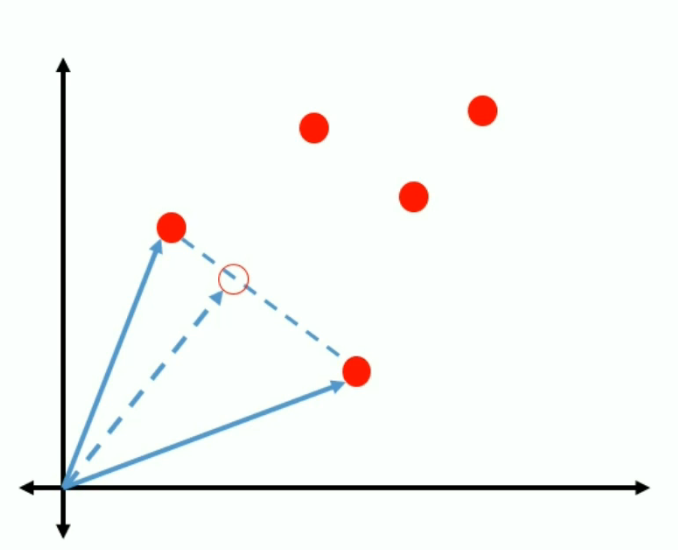
\includegraphics[scale=0.25]{smote.png}\\
				\caption{Creazione di un nuovo dato sintetico con SMOTE}
				\label{smote_fig}
			\end{figure}
			
			\subsection{Synthetic Minority Oversampling Technique} \label{sec:smote}
				SMOTE (Synthetic Minority Oversampling Technique) è una tecnica di oversampling che invece di replicare gli stessi dati più volte ne crea di nuovi basandosi sulle feature di dati già esistenti \cite{smote}. Preso in modo casuale un dato $x$ appartenente alla classe che si vuole aumentare, gli si applica l'algoritmo \textbf{k-nearest neighbors} che trova i $k$ campioni più vicini a $x$ nel dataset. Come si può osservare in figura 2.4 si genera un nuovo punto in modo che questo giaccia sul segmento che congiunge $x$ e uno dei $k$ vicini. %\ref{fig:smote_fig} < non funziona.


				
				
	\chapter{Esperimenti} \label{chap:esperimenti}
		In questo Capitolo verranno trattati alcuni esperimenti con le \textbf{reti neurali} utilizzando le tecniche viste nel Capitolo 2. L'idea di questo lavoro è stata quella di familiarizzare inizialmente con i percettroni multistrato attraverso \texttt{MLPClassifier} di sklearn \cite{sklearn}. Si è poi passati a cercare di massimizzare l'accuratezza del classificatore tramite delle tecniche di \textbf{preprocessing} e \textbf{model selection}, per poi infine fare esperimenti sull'aumento dei dati per vedere come crescerebbe ipoteticamente l'accuratezza con l'aumentare della numerosità del dataset.
	
	\section{Dataset} 
		In questo paragrafo verrà fatta una panoramica sui dataset utilizzati durante gli esperimenti. Prima di entrare nei dettagli con gli esperimenti di classificazione, reingegnerizzazione dei dati e data augmentation verrà fatta un'analisi visiva dei dati per avere un'idea di come essi siano composti e quali tecniche di preprocessing necessitino.  Le tecniche di visualizzazioni principali utilizzate saranno il \textbf{box plot} e lo \textbf{scatter plot}. 
		\begin{table}[h]
			\noindent\makebox[\textwidth]{
			\begin{tabular}{ccccc}
			\toprule
			sepal length &  sepal width &  petal length &  petal width &        type \\
			\midrule
			4.8 &               3.4 &                1.6 &               0.2 &      setosa \\
			6.5 &               3.0 &                5.5 &               1.8 &   virginica \\
			6.1 &               2.8 &                4.0 &               1.3 &  versicolor \\
			\bottomrule
			\end{tabular}}
			\caption{\label{tab:iris}Tre misurazioni appartenenti all'iris dataset.}
		\end{table}
			
		\subsection{Iris dataset}
			Il primo dataset utilizzato per fare esperimenti e familiarizzare con \texttt{MLPClassifier} è stato \textbf{iris dataset}. Questo insieme di dati raccoglie 150 istanze, 50 per ciascuna specie dei tre fiori iris presenti: \textit{iris setosa, iris virginica} e \textit{iris versicolor}. Per ogni campione oltre all'etichetta sono presenti la lunghezza e la larghezza del sepalo e del petalo in centimetri. Questo dataset è ampiamente utilizzato come primo esempio nel mondo del machine learning in quanto presenta dei dati che praticamente non hanno bisogno di essere preelaborati. I box plot in figura \ref{fig:boxplot_iris} ci permettono di osservare le distribuzioni di ogni feature e gli outlier; i dati si distribuiscono tutti su un range abbastanza simile, quindi in questo caso non c'è la necessità di standardizzare i dati. Nella feature \textit{sepal width} gli outlier non sono troppo distanti dalla mediana, quindi non sono da considerarsi fastidiosi. È interessante vedere anche i diagrammi di dispersione che ci sono tra le diverse combinazioni di attributi: essi ci aiutano a capire quanto due feature siano correlate tra di loro, e potrebbe tornare utile per
			\begin{itemize}
				\item aiutare a predire un attributo da un altro (ottimo modo per imputare valori mancanti o errati),
				\item indicare (non sempre) la presenza di relazioni di causa-effetto.
			\end{itemize}
			Inoltre distinguendo per colore la classe di appartenenza di ogni dato come in figura \ref{fig:scatter_iris}  ci si può accorgere se i dati sono separabili linearmente e si potrebbe decidere di utilizzare una funzione lineare invece che un modello di machine learning. Ad esempio, se volessimo discriminare solo gli \textit{iris setosa} dagli altri due fiori ci basterebbe tracciare una retta che separa i dati. In questo dataset avendo solo 4 feature ridurre le dimensionalità con PCA e t-SNE non porta grossi vantaggi, come si può notare in figura \ref{fig:pca_tsne_iris} i grafici ottenuti non sono tanto diversi da quelli che si potevano vedere in precedenza.
			
			\img{Box plot dei dati dell'iris dataset}{0.5}{boxplot.png}{boxplot_iris}
			\img{Scatter plot di ogni combinazione di feature dell'iris dataset. Nella diagonale della matrice è tracciata la distribuzione della feature divisa per classe.}{0.6}{scatter.png}{scatter_iris}
			
			\begin{figure}
				\begin{subfigure}[]{.5\textwidth}
					\centering
					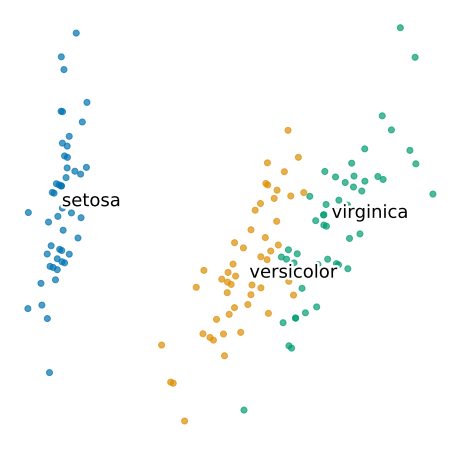
\includegraphics[width=.9\linewidth]{iris_pca.png}
					\caption{PCA}
					\label{fig:iris_pca}
				\end{subfigure}
				\hfill
				\begin{subfigure}[]{.5\textwidth}
					\centering
					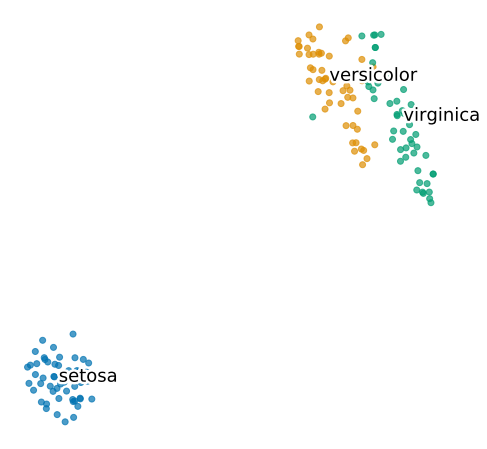
\includegraphics[width=.9\linewidth]{iris_tsne.png}
					\caption{t-SNE}
					\label{fig:iris_tsne}
				\end{subfigure}
				
				\caption{Riduzione della dimensionalità dell'iris dataset}
				\label{fig:pca_tsne_iris}
			\end{figure}	

			
		\subsection{Dataset sugli incidenti stradali} \label{sec:incidenti}
			Il dataset sugli incidenti stradali è l'insieme di dati su cui è stato svolto il lavoro principale di questo tirocinio. Sono presenti 130 campioni riguardanti incidenti stradali in cui sono stati coinvolti dei pedoni. Ogni riga è identificata da un \textit{verbale} e sono presenti la data in cui è avvenuto l'incidente, i dati personali della vittima, dei dati sulle lesioni occasionate in 20 aree diverse del corpo e infine, la tipologia di mezzo che ha occasionato l'incidente che può essere 0 \textit{(leggero)} o 1 \textit{(pesante)}. I dati personali sono \textit{sesso, anni, peso, altezza} e \textit{BMI}, mentre i dati sulle lesioni sono relativi a 4 macroaree quali \textit{testa, torace, addome} e \textit{scheletro}. Per ognuna di esse sono presenti 5 aree specifiche con un valore di gravità della lesione che va da 0 a 4. Sono inoltre presenti anche i totali per ogni macroarea che sono la somma delle loro 5 aree specifiche, più un totale per tutto il corpo che è una somma complessiva dei 20 dati sulle lesioni. 
			\begin{table}[h]
			\begin{tabular}{lccccccc}
			\toprule
			VERBALE & DATA &  SESSO &  ANNI & $\dots$ &  Tot Addome &  Tot Scheletro &  Totale \\
			\midrule
			85567 & 1999-10-29 &      0 &    81 &  $\dots$ &         3 &              9 &      14 \\
			85829 & 2000-01-14 &      1 &    69 &  $\dots$ &         1 &              4 &      32 \\
			85977 & 2000-03-10 &      1 &    71 &  $\dots$ &         0 &              4 &      10 \\
			86220 & 2000-06-14 &      1 &    54 &  $\dots$ &         2 &              4 &      14 \\
			86247 & 2000-06-22 &      1 &    78 &  $\dots$ &         2 &              4 &       8 \\
			\bottomrule
			\end{tabular}
			\caption{\label{tab:incidenti}Prime 5 righe del dataset sugli incidenti stradali.}
			\end{table}
			
			Come possiamo vedere dalla tabella \ref{tab:incidenti} la data non è un dato numerico, va quindi convertito tramite feature encoding: in questo caso si è scelto semplicemente di trasformare la data nel numero di giorni passati dall'epoca \texttt{unix} (01/01/1970). Osservando i diagrammi di dispersione in figura~\ref{fig:scatter_incidenti} si può notare come i dati con etichetta diversa siano molto più mischiati rispetto al dataset visto in precedenza (figura \ref{fig:scatter_iris}). Una cosa che salta all'occhio osservando gli scatter plot in cui è convolta la data (figura \ref{fig:scatter_data}) è che c'è un cluster di dati in cui il mezzo è pesante quando la data assume valori bassi. Infatti, se si ordinano i dati in base alla data, si può notare che le prime 24 righe hanno come etichetta \texttt{Mezzo} un valore pari a 1 \textit{(eccetto la prima riga, nella figura \ref{fig:scatter_data} questo dato corrisponde al pallino blu più basso)}. Ovviamente questo potrebbe essere un problema per la rete neurale, in quanto il dato che sembra discriminare meglio l'etichetta è quello relativo a una variabile che in realtà non dovrebbe dirci niente sul tipo di mezzo che ha causato l'incidente. Durante gli esperimenti si terrà conto di questo fatto, e nella maggior parte di essi si eliminerà l'intera colonna. 
			
			\img{Scatter plot di DATA e BMI}{0.4}{scatter_data.png}{scatter_data}
			
			Come possiamo vedere in figura \ref{fig:pca_tsne_incidenti}, riducendo la dimensionalità dei dati con PCA e t-SNE i dati restano molto mischiati, quindi possiamo aspettarci di non avere delle performance altissime, soprattuto data la numerosità del dataset.
			
			\begin{figure}[h]
				\begin{subfigure}[]{.5\textwidth}
					\centering
					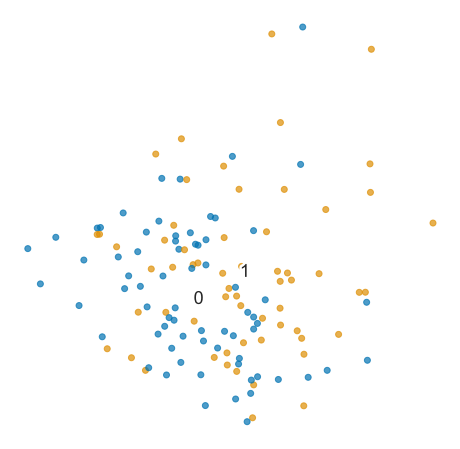
\includegraphics[width=.7\linewidth]{pca_incidenti.png}
					\caption{PCA}
					\label{fig:pca_incidenti}
				\end{subfigure}
				\hfill
				\begin{subfigure}[]{.5\textwidth}
					\centering
					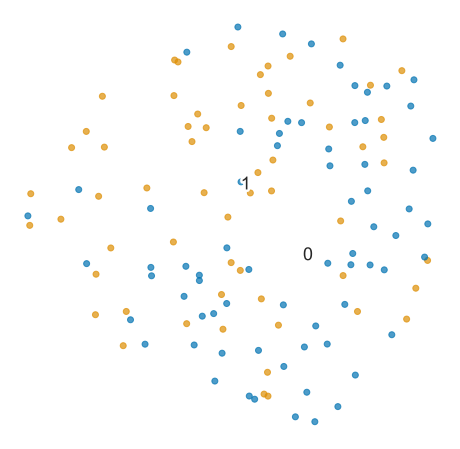
\includegraphics[width=.7\linewidth]{tsne_incidenti.png}
					\caption{t-SNE}
					\label{fig:tsne_incidenti}
				\end{subfigure}
				
				\caption{Riduzione della dimensionalità del dataset sugli incidenti}
				\label{fig:pca_tsne_incidenti}
			\end{figure}	
			\img{Scatter plot di ogni combinazione di feature dataset sugli incidenti. Nella diagonale della matrice è tracciata la distribuzione della feature divisa per classe.}{0.25}{scatter_incidenti.png}{scatter_incidenti}
 				
	\section{Classificazione e reingegnerizzazione dei dati} 
		Dopo aver dato uno sguardo generale ai dati su cui si dovrà lavorare, si può iniziare a fare esperimenti di classificazione e reingegnerizzazione dei dati. Inizialmente verranno mostrati i primi esperimenti utilizzati per familiarizzare con \texttt{MLPClassifier} e l'iris dataset, per poi passare agli esperimenti sul dataset degli incidenti stradali. 
		
		\subsection{Iris Dataset}
			Il primo esperimento di classificazione fatto con questo dataset è stato quello di provare a creare un percettrone multistrato impostando alcuni iperparametri in modo casuale per poi allenarlo con un insieme di train e testarlo con un insieme di test. Il tutto è stato fatto senza fare nessun tipo di preprocessing e model selection, infatti l'accuracy ottenuta è molto bassa. Confrontando le etichette predette con quelle che ci si aspettava di ottenere (codice \ref{lst:iris_1}) ci si accorge presto che c'è stato un problema nella fase di apprendimento. 

			\begin{lstlisting}[language=Python, caption=Primo esperimento con l'iris dataset, captionpos=t, gobble=8, label={lst:iris_1}]
				from sklearn.model_selection import train_test_split
				from sklearn.neural_network import MLPClassifier
				
				X_train, X_test, y_train, y_test = train_test_split(X, y)
				
				nn = MLPClassifier(activation='logistic', hidden_layer_sizes=(2), learning_rate_init=0.5, max_iter=500)
				
				nn.fit(X_train, y_train)
				
				print("Accuracy: %0.2f" % nn.score(X_test, y_test))
			\end{lstlisting}
			\texttt{Accuracy: 0.26}
			
			 
			\begin{lstlisting}[language=Python, gobble=8]
				nn.predict(X_test)
			\end{lstlisting}
			\texttt{array([2, 2, 2, 2, 2, 2, 2, 2, 2, 2, 2, 2, 2, 2, 2, 2, 2, 2, 2, 2, 2, 2, 2, 2, 2, 2, 2, 2, 2, 2, 2, 2, 2, 2, 2, 2, 2, 2])}
			
			\begin{lstlisting}[language=Python, gobble=8]
				y_test
			\end{lstlisting}
			\texttt{array([1, 1, 0, 2, 1, 1, 2, 2, 1, 2, 1, 2, 2, 2, 2, 0, 2, 0, 2, 2, 2, 2, 1, 0, 0, 0, 0, 0, 0, 0, 1, 1, 2, 2, 0, 0, 1, 2])}\\\\
			Osservando i dati ci si è accorti che essi hanno poco bisogno di essere preelaborati, quindi si è subito provata una tecnica di model selection. Si è deciso di fissare come funzione di attivazione la funzione logistica e 500 come numero massimo di iterazioni, per poi applicare la \texttt{GridSearchCV} con $k=5$ per la cross validation, testando le combinazioni dei seguenti iperparametri:
			\begin{itemize}
				\item \texttt{hidden\_layer\_sizes: [(10,2), (10), (5,5)]} \textit{(L'i-esimo elemento di una tupla rappresenta il numero di neuroni nello strato nascosto i)},
	    		\item \texttt{learning\_rate\_init: [0.2, 0.1, 0.01]} \textit{(learning rate \textbf{iniziale}, in quanto esistono tecniche in cui esso varia durante la fase di apprendimento)}
			\end{itemize}
			In questo modo si è ottenuta una rete neurale in cui la combinazione di iperparametri migliore è risultata essere quella con 10 neuroni in un singolo strato nascosto e un learning rate pari a 0.2. L'accuratezza conseguita sul test set con questi iperparametri è  stata del 99\%. Si è poi utilizzata una cross validation annidata con $k = 3$ esterno e $k' = 5$  interno per testare la bontà di generalizzazione in modo più imparziale, e si è ottenuta una accuratezza pari al 97\% con una deviazione standard di +/- 0.05. Questi risultati confermano che questo	dataset non necessiti di una fase di preprocessing.
			
		\subsection{Dataset sugli incidenti stradali}
			Come abbiamo già visto nel paragrafo \ref{sec:incidenti}, i dati sulle lesioni sono diversi e quindi nel dataset è presente un totale per ogni macroarea. Quando si è andati a fare i primi esperimenti di classificazione, si è notato che mantenendo sia il totale che le singole lesioni la accuratezza del classificatore era più bassa rispetto a quando si escludeva una delle due informazioni. Probabilmente questo è dovuto alla ridondanza dei dati, quindi sono stati fatti degli esperimenti testando l'accuratezza di diversi percettroni multistrato per capire se fosse meglio mantenere i totali o le 20 singole lesioni. I risultati hanno dimostrato che conservare solo i totali aumentasse leggermente le prestazioni, pertanto nei seguenti esperimenti si è stabilito di mantenere solo la somma delle lesioni per le diverse macroaree e poi di provare tecniche di riduzione della dimensionalità diverse dalla somma.
			
			\subsubsection{Data o non data?}			
				È già stato spiegato nel paragrafo \ref{sec:incidenti} perchè l'elemento \texttt{DATA} si ritenga debba essere escluso, ma è curioso osservare quanto cambi l'accuratezza di un percettrone multistrato con e senza questa feature. Sono stati considerati due insiemi \texttt{X} e \texttt{X\_no\_data} in cui erano presenti tutte le righe del dataset, in \texttt{X} era presente la feature \texttt{DATA} mentre nell'altro insieme no. La preelaborazione fatta sui dati dei due insiemi per questo esperimento è stata: 
				\begin{itemize}
					\item eliminare i dati delle singole lesioni,
					\item applicare una scalatura standard sui dati.
				\end{itemize}
				La scalatura standard è stata applicata poichè i dati sono distribuiti in modo molto diverso tra di loro; basti pensare alla differenza che c'è tra la data \textit{(dopo la procedura di feature encoding)} e i dati sulle singole lesioni. Ad esempio nella Tabella \ref{tab:differenza_data} vi è una comparazione tra la media, la deviazione standard, il valore minimo, massimo e alcuni percentili tra la colonna contenente le date e le lesioni al cuore.
				
				\begin{table}
				\centering
				\begin{tabular}{lrr}
				\toprule
				{} &          DATA &  Torace:Cuore \\
				\midrule
				count &    130.0 &    130.0 \\
				mean  &  14945.8 &      0.5 \\
				std   &   1880.8 &      0.9 \\
				min   &  10893.0 &      0.0 \\
				25\%   &  13453.7 &      0.0 \\
				50\%   &  15198.0 &      0.0 \\
				75\%   &  16282.5 &      1.0 \\
				max   &  18030.0 &      4.0 \\
				\bottomrule
				\end{tabular}
				\caption{Comparazione dei dati di due colonne del dataset}
				\label{tab:differenza_data}
				\end{table}
				
				Dopo la preelaborazione dei dati è stata svolta una fase di model selection per trovare il miglior classificatore per ognuno dei due insiemi e per compararne le prestazioni. Si è eseguita una cross validation annidata per testare diverse combinazioni di iperparametri, tra cui: 
			\begin{itemize}
				\item \texttt{max\_iter: [100,1000,5000],}
	          	\item \texttt{hidden\_layer\_sizes: [[2], [4], [6], [10], [20], [4, 4], [10, 10]],}
	          	\item \texttt{learning\_rate\_init : [0.01, 0.2, 0.001],}
	          	\item \texttt{activation: [logistic, tanh, relu].}
			\end{itemize}
			I classificatori ottenuti tramite la feature selection sono abbastanza simili, ma come ci si poteva aspettare, lo score ottenuto con la feature \texttt{DATA} presente è leggermente più alto (Tabella \ref{tab:score_con_e_senza_data}). 

			\begin{table}
				\centering
				\begin{tabular}{lcccccc}
				\toprule
				 & Activation &  Learning rate & Hidden layer sizes &  Max iter &    Best score &  Test score \\
				\midrule
				X &       tanh &               0.010 &                [2] &       100 &  0.756 &    0.727 \\
				X\_no\_data &      tanh &               0.001 &                [2] &      5000 &  0.749 &    0.697 \\
				\bottomrule
				\end{tabular}
				\caption{Comparazione delle accuratezze ottenute con e senza la feature \texttt{DATA}. La colonna \textit{Best score} rappresenta il miglior score ottenuto nella cross validation interna, mentre \textit{Test score} rappresenta lo score ottenuto con la cross validation esterna.}
				\label{tab:score_con_e_senza_data}
			\end{table}	
			
			\subsubsection{Utilizzo di tecniche di riduzione della dimensionalità per il calcolo dei totali} \label{par:pca_totali}
				Un altro esperimento svolto è stato quello di utilizzare gli algoritmi di riduzione della dimensionalità \textbf{PCA} e \textbf{t-SNE} per provare a ridurre le singole lesioni in un numero minore di colonne con una tecnica che fosse diversa dalla somma, sostituendo così i totali. Con t-SNE si sono ottenuti risultati molto simili a quelli già avuti in precedenza, mentre riducendo a 2 dimensioni le lesioni per ogni macroarea del corpo con PCA si sono ottenute performance leggermente migliori. Anche in questo esperimento sono stati esclusi l'attributo \texttt{DATA} e i dati sulle singole lesioni che sono stati utilizzati per calcolare la PCA. Non è stata fatta una vera e propria model selection, bensì sono stati fissati un \textit{learning rate} pari a 0.001 e un numero massimo di iterazioni pari a 5000, per poi osservare l'accuracy cross validata con $k=5$ di tutte le combinazioni di: 
				\begin{itemize}
					\item \texttt{activations: [relu, logistic, tanh],}
    				\item \texttt{hidden\_layers = [(2), (3,3), (5), (6,3), (5,5), (6), (8), (10), (2,2,2)].}
				\end{itemize}
				Sono state disposte su una tabella tutte le accuratezze della cross validation, l'accuratezza media e la deviazione standard per ogni combinazione tra funzione di attivazione e neuroni negli strati nascosti, ordinandoli in ordine crescente. Come è possibile vedere nelle Tabelle \ref{tab:totali_somma} e \ref{tab:totali_pca} l'accuratezza media passa da un massimo di 0.70 a 0.73. È interessante notare che in entrambi i casi, la funzione di attivazione logistica sembra avere la meglio in quanto compare molto più spesso delle altre due tra i primi 5 risultati.
				\begin{table}
					\begin{tabular}{lllrr}
					\toprule
					Activation & Hidden layer sizes &                               Scores &  Mean score &  Scores std \\
					\midrule
					logistic &                  5 &  [0.654, 0.731, 0.769, 0.808, 0.538] &       0.700 &       0.095 \\
					tanh &             (6, 3) &  [0.654, 0.692, 0.769, 0.769, 0.538] &       0.685 &       0.086 \\
					logistic &                  8 &    [0.615, 0.692, 0.769, 0.808, 0.5] &       0.677 &       0.110 \\
					logistic &                  6 &  [0.654, 0.731, 0.808, 0.654, 0.538] &       0.677 &       0.090 \\
					logistic &             (6, 3) &  [0.654, 0.769, 0.577, 0.808, 0.577] &       0.677 &       0.096 \\
					\bottomrule
					\end{tabular}
					\caption{Primi 5 risultati ottenuti con la somma come totali.}
					\label{tab:totali_somma}
				\end{table}
				\begin{table}
					\begin{tabular}{lllrr}
					\toprule
					Activation & Hidden layer sizes &                               Scores &  Mean score &  Scores std \\
					\midrule
					logistic &                  6 &  [0.769, 0.577, 0.769, 0.808, 0.731] &       0.731 &       0.081 \\
					logistic &                  5 &  [0.692, 0.654, 0.769, 0.808, 0.654] &       0.715 &       0.062 \\
					logistic &                  8 &  [0.731, 0.654, 0.731, 0.769, 0.654] &       0.708 &       0.046 \\
					tanh &             (6, 3) &  [0.615, 0.654, 0.731, 0.769, 0.731] &       0.700 &       0.057 \\
					logistic &                 10 &  [0.654, 0.615, 0.769, 0.769, 0.692] &       0.700 &       0.062 \\
					\bottomrule
					\end{tabular}
					\caption{Primi 5 risultati ottenuti con PCA come totali.}
					\label{tab:totali_pca}
				\end{table}
	
	\section{Data augmentation}
		Tutti gli esperimenti di questa sezione sono stati svolti sul dataset degli incidenti stradali. Dopo aver svolto diversi esperimenti sulla reingegnerizzazione dei dati osservando l'accuratezza del classificatore per ognuno di essi, si è notato che sopra un certo limite $(\sim 0.75)$ l'accuratezza non sale. Una rete neurale per generalizzare bene dei dati deve avere a disposizione un'elevata quantità di dati, soprattutto se essi appartengono a un dataset in cui i dati appartenenti alle diverse classi sono mischiati come in questo caso.  Si è deciso di provare a fare degli esperimenti di \textbf{data augmentation} per avere un'idea di come l'accuratezza potrebbe ipoteticamente variare in caso si disponesse di più dati.
		
		\subsection{Data augmentation con SMOTE} \label{sec:data_aug_smote}
			Il primo esperimento di data augmentation è stato svolto con la tecnica di over sampling \textbf{SMOTE} spiegata nel paragrafo \ref{sec:smote}. A partire dall'insieme originale sono stati creati diversi insiemi di dati sintetici, aumentando sempre di più la cardinalità, per poi applicare un processo di model selection ad ogni insieme. I modelli ricavati da questo processo, essendo stati allenati con dati fittizi non sono applicabili nella pratica. 
			
			Anche in questo caso ai dati sono state rimosse le feature \texttt{DATA} e le 20 lesioni singole prima di applicare SMOTE. I dati sono stati incrementati da 130 a 200, 300, $\dots,$ 2000 sempre con uno step di 100. Raggiunta una certa cardinalità, l'accuratezza tendeva a stabilizzarsi, quindi dopo i 2000 si è deciso di crescere in modo esponenziale (fino a $2^{16}$). Per ogni insieme si è applicata la seguente procedura:
				\begin{itemize}
				 \item sono stati standardizzati i dati tramite la scalatura standard,
				 \item si è fatta una model selection tramite \texttt{GridSearchCV}, fissando il \textit{learning rate} a 0.001 e il numero massimo di iterazioni a 5000, dividendo l'insieme in 5 parti per la cross validation e testando gli iperparametri:
				 	\begin{itemize}
					\item \texttt{activations: [relu, logistic, tanh],}
    				\item \texttt{hidden\_layers = [(2), (3,3), (5), (6,3), (5,5), (6), (8), (10).}
					\end{itemize}
				 \end{itemize}
			In questo procedimento, per quasi ogni insieme la rete migliore ottenuta con il processo di model selection è stata quella con funzione di attivazione \texttt{tanh} e 10 neuroni in un singolo strato nascosto. Le accuratezze ottenute con gli insiemi più numerosi sono arrivate oltre lo 0.96 (Figura \ref{fig:accuracy_smote}). Si è notato che i neuroni nello strato nascosto di tutte le reti che hanno avuto i risultati migliori erano 10, che è il numero massimo di neuroni messi per la model selection. Si è quindi deciso di provare ad aumentare questo numero fino a 50, ottenendo risultati migliori (si è arrivati ad ottenere accuratezze oltre lo 0.99 per gli insiemi più numerosi), ma avere un rapporto così diverso tra neuroni di ingresso, che nel nostro caso sono 9 dato che stiamo lavorando con 9 colonne, e neuroni nello strato nascosto potrebbe portare all'\textbf{overfitting} molto più facilmente.
			\imgh{Grafico che mostra il crescere dell'accuratezza all'aumentare della numerosità dell'insieme con SMOTE. Il grafico sotto è un ingrandimento del primo.}{0.35}{accuracy_smote_1.png}{accuracy_smote}
			
		\subsection{Data augmentation con perturbazione sui dati personali} \label{sec:data_aug_pers}
			Un altro esperimento di data augmentation svolto è stato quello di creare nuovi dati basandosi su campioni già esistenti nel dataset originale perturbando solo i dati personali con distribuzione normale, ovvero \texttt{ANNI}, \texttt{PESO} e \texttt{ALTEZZA}, ricalcolando il BMI a partire dai nuovi dati generati secondo la formula \texttt{BMI = PESO / ALTEZZA$^2$} e lasciando fissi i dati sulle lesioni. I dati sono stati perturbati nel seguente modo: 
			\begin{itemize}
			\item ad \texttt{ANNI} è stata aggiunta una perturbazione estratta da una distribuzione normale con media pari a 0 e deviazione standard pari a 1, arrotondata al numero intero più vicino,
			\item a \texttt{PESO} (kg) è stata aggiunta una perturbazione estratta da una distribuzione normale con media pari a 0 e deviazione standard pari a 2 kg,
			\item ad \texttt{ALTEZZA} (m) è stata aggiunta una perturbazione estratta da una distribuzione normale con media pari a 0 e deviazione standard pari a 1 cm.
			\end{itemize}
			Dal dataset è stata eliminata la feature \texttt{DATA}, le lesioni singole e i totali, per poi ricalcolarli con PCA come spiegato nel sottoparagrafo \textit{\say{Utilizzo di tecniche di riduzione della dimensionalità per il calcolo dei totali}} presente nel paragrafo \ref{par:pca_totali}. Per ogni insieme si è applicata la seguente procedura:
				\begin{itemize}
				\item sono stati ricalcolati i totali con PCA passando a 2 dimensioni,
				\item sono stati standardizzati i dati tramite la scalatura standard,
				\item si è fatta una model selection tramite \texttt{GridSearchCV}, fissando il \textit{learning rate} a 0.001 e il numero massimo di iterazioni a 5000, dividendo l'insieme in 5 parti per la cross validation e testando gli iperparametri:
				 	\begin{itemize}
					\item \texttt{activations: [relu, logistic, tanh],}
    				\item \texttt{hidden\_layers = [(2), (3,3), (5), (6,3), (5,5), (6), (8), (10), (20).}
					\end{itemize}
				 \end{itemize}
			Con questo esperimento di data augmentation la rete che ottiene più comunemente i risultati migliori ha come funzione di attivazione la \texttt{tanh} e questa volta 20 neuroni in un singolo strato nascosto, che nell'esperimento di prima erano assenti. In questo caso va fatto notare che avendo calcolato i totali con PCA riducendo a 2 le dimensioni per ogni macroarea delle lesioni, si ha un dataset con 13 colonne, quindi si hanno 13 neuroni di ingresso. Le accuratezze raggiunte con questo esperimento sono più alte, già con 700 dati si raggiunge un'accuratezza molto vicina a 1 (Figura \ref{fig:accuracy_data_aug_pers}).
			
			\img{Grafico che mostra il crescere dell'accuratezza all'aumentare della numerosità dell'insieme perturbando i dati personali. Il grafico sotto è un ingrandimento del primo.}{0.35}{accuracy_data_aug_pers.png}{accuracy_data_aug_pers}
			
			\paragraph{Feature selection} Dopo aver aumentato i dati è stata svolta un'attività di feature selection sui dati personali per vedere se tutti i dati fossero essenziali. //QUESTA PARTE È DA CONCLUDERE

		\subsection{Data augmentation con perturbazione sui dati appartenenti alle lesioni} \label{sec:data_aug_les}
			Dopo aver aumentato i dati basandosi su campioni già esistenti perturbando i dati personali continui, si è provato a ripetere l'esperimento ma questa volta perturbando i dati sulle lesioni e lasciando invariati i dati personali. I dati relativi alle lesioni sono più sensibili in quanto è difficile stabilire se una perturbazione sia stata fatta in modo corretto, si è quindi deciso di perturbare i dati in modo leggero, applicando casualmente a solo 3 tra le 20 colonne relative alle lesioni una perturbazione di $-2, -1, 0, 1, 2$ con rispettiva probabilità $0.1, 0.2, 0.4, 0.2, 0.1$, sempre restando nel range accettabile dalle singole lesioni $[0,4]$. Il preprocesing dei dati e la model selection sono stati eseguiti esattamente come nell'esperimento prima (Paragrafo \ref{sec:data_aug_pers}) e anche in questo caso la rete migliore più più frequente ha come funzione di attivazione la \texttt{tanh} e 20 neuroni in un singolo strato nascosto. Anche in questo esperimento le accuratezze tendono a incrementare con l'aumentare della numerosità del dataset, con la differenza che oltre un certo numero tende a decrescere per poi crescere nuovamente (Figura \ref{fig:accuracy_data_aug_lesioni}). 
			\img{Grafico che mostra il variare dell'accuratezza all'aumentare della numerosità dell'insieme perturbando i dati sulle lesioni. Il grafico sotto è un ingrandimento del primo.}{0.35}{accuracy_data_aug_lesioni.png}{accuracy_data_aug_lesioni}
			
		\subsection{Data augmentation con perturbazione sui dati personali e sui dati appartenenti alle lesioni}
			Dopo aver svolto i due esperimenti di data augmentation in cui sono stati creati nuovi dati a partire da elementi già esistenti nel dataset perturbando prima i dati personali (Paragrafo \ref{sec:data_aug_pers}) e poi le lesioni (Paragrafo \ref{sec:data_aug_les}), si è deciso di unire i due esperimenti per osservarne i risultati. Il processo di preprocessing e model selection è il medesimo degli esperimenti sopracitati, così come anche la miglior rete più frequente. Anche in questo caso si può notare in figura \ref{fig:acc_data_aug_both} una decrescita dell'accuratezza dopo aver raggiunto un certo numero di dati (intorno agli 800/1000).
			\img{Grafico che mostra il variare dell'accuratezza all'aumentare della numerosità dell'insieme perturbando i dati personali e i dati sulle lesioni. Il grafico sotto è un ingrandimento del primo.}{0.35}{acc_data_aug_both_.png}{acc_data_aug_both}
			
			
			
	\chapter*{Conclusione}	\addcontentsline{toc}{chapter}{Conclusione}  
	
	\begin{thebibliography}{9}
		\bibitem{kriesel} David Kriesel, 2007, \textit{A Brief Introduction to Neural Networks}, available at \texttt{http://www.dkriesel.com}.

		\bibitem{shwartz} Shai Shalev-Shwartz, Shai Ben-David, 2014, \textit{Understanding Machine Learning: From Theory to Algorithms}, Cambridge University Press.
		
		\bibitem{mcculloch_pitts} Warren S. McCulloch, Walter Pitts, 1943, \textit{A logical calculus of the ideas immanent in nervous activity}, The bulletin of mathematical biophysics volume 5.		
		
		\bibitem{minsky_papert} Marvin Minsky, Seymour Papert, 1969,  \textit{Perceptrons: an introduction to computational geometry}, Information and control 17, 501-522- 
		
		\bibitem{bitsofdna} Bits of DNA, \texttt{https://liorpachter.wordpress.com/}.
		
		\bibitem{maaten_hinton} Laurens van der Maaten, Geoffrey Hinton, 2008, \textit{Visualizing Data using t-SNE}, Journal of Machine Learning Research 9, 2579-2605.
		
		\bibitem{sklearn} Scikit-learn, \texttt{https://scikit-learn.org/}.
		
		\bibitem{smote} Nitesh V. Chawla, Kevin W. Bowyer, Lawrence O. Hall, W. Philip Kegelmeyer, 2002, \textit{SMOTE: Synthetic Minority Over-sampling Technique}, Journal of Artificial Intelligence Research 16, 321–357.
		
		\bibitem{neyman} Jerzy Neyman, 1934, \textit{On the Two Different Aspects of the Representative Method: The Method of Stratified Sampling and the Method of Purposive Selection}, Journal of the Royal Statistical Society Vol. 97, No. 4.
		
	\end{thebibliography}
	
\end{document}



